\documentclass{article}
\usepackage{silence}
\WarningsOff*
\usepackage{graphicx} % Required for inserting images
\usepackage[numbers]{natbib}
\usepackage{url}
\setlength{\parskip}{\baselineskip}
\usepackage{hhline} 


\title{Indication of the appraisal in the moment on the appraisal in the memory}
\author{Taichi Uno}
\date{December 2023}
\begin{document}

\maketitle

\begin{abstract}
    % One of the challenges in the field of intelligent systems is to understand how individuals subjectively perceive situations during interactions. Concepts like the appraisal process and situation perception serve as frameworks for systematically assessing situations and conversation partners in cognitive science. Situational interdependence, a facet of situation perception, measures how an individual perceives a situation influencing both their and others' outcomes. This research aims to fill gaps in understanding how the appraisal process shapes an individual's summary evaluation of situational interdependence by modelling a representation of the appraisal process from textual content and non-textual verbal cues and how the context settings of conversation play roles here. Success in this research contributes to broadening the scope of researching the appraisal process from a computational point of view and potentially leads to a more sophisticated way of automatically recognizing a user's perceived situational interdependence across various contexts.
\end{abstract}

\section{Introduction} \label{intro}
% Understanding of human appraisal is useful for intelligent systems
One of the challenges in the field of intelligent systems is to understand how individuals subjectively appraise situations in interactions. Appraisal is defined as the process of evaluating situations based on personal belief, relevance, and significance \cite{scherer2005emotions}. This type of information is particularly beneficial for adaptive intelligence systems where they try to change their behaviours and responses such that they fit a user at a specific moment in time. A better understanding of users' perception of a situation is necessary to make the learning process more effective by identifying the specific pattern, phenomenon or social signals that can be utilized for inference of human perception. Traditionally, psychologists try to structurally uncover the process of how one perceives and evaluates a situation from different perspectives to understand different aspects of a situation, such as emotions \cite{scherer2005emotions, scherer2013nature}, situation perception \cite{rauthmann2014situational}, or situational interdependence \cite{gerpott2017howdopeople}.

% back up with literature, write stuff down, explainability, definition of "appraisal"

% Appraisal as remembered
%     After an interaction, one reappraises the situation by recalling what it was like. (To be defined more clearly)
%     Usually measured by post-interaction questionnaire
% Appraisal in the moment
%     Real-time appraisal of a situation during an interaction.  (To be defined more clearly)
%     Have not attempted to collect much yet.
As stated earlier, appraisal refers to the assessment process of situations based on personal beliefs, relevance, and significance \cite{scherer2005emotions}. The cognitive process of evaluation can be described by a set of appraisal variables/dimensions. The theories of appraisal are currently vague in how time plays a role and the dynamics of appraisal due to changes in situations, instead, they focus on classifying emotional reactions or cognitive evaluation of situations based on different dimensions. Therefore, the present research clearly distinguishes two appraisals based on the moment of appraisal and the stimulus events. Appraisal in the moment is defined as appraisal that is carried out in the moment of events. It is closely related to the concept of appraisal dynamics, which captures evolving situations and evaluates appraisal variables dynamically \cite{marsella2009ema}. On the other hand, appraisal as remembered is defined as appraisal of past events. This is attained from reappraisal of the past event by evaluating the mental recollection of happened events or recalling appraisal variables. The cognitive process of these two are different and it is expected to be dependent on how the recall was initiated (e.g. how the triggering prompt is formulated \cite{FIND A SOURCE!}.

% One example is situation perception and situational interdependence 
As an example of different aspects of appraisal, situation perception is a type of cognitive process that interprets and understands situations subjectively based on an individual's experiences, beliefs, and expectations \cite{tekoppele2023we}. The expressed emotions and behaviour can be indicative of how one perceives a situation \cite{hess2020bidirectional, horstmann2019situational}. When it comes to different aspects of evaluation, as one of the facets of situation perception, there is situational interdependence, which particularly highlights the perceived interdependence in a certain situation. The situational Interdependence Scale (SIS) proposed by \citeauthor{gerpott2017howdopeople} \cite{gerpott2017howdopeople} provides a way to quantify subjective (or perceived) interdependence based on the five dimensions (mutual dependence, conflict of interest, future independence, information certainty, and power) that articulate individuals' perceptions of their interdependence. 

\begin{table}
    \centering
    \begin{tabular}{|c|l|} \hline
        Dimension & Description\\\hline
       Mutual Dependence  & \\
       Conflict of Interest  & \\
       Future Independence  & \\
       Information Certainty  & \\
       Power  & \\ \hline
    \end{tabular}
    \caption{Dimensions of situational interdependence \cite{gerpott2017howdopeople}}
    \label{tab:sis_dimensions}
\end{table}

% Another example is Appraisal process of emotion
Another specific example of different aspects of cognitive appraisal, the component process model (CPM) of appraisal is inherited from the appraisal theory of emotion, in which specific configurations of those dimensions in combination define emotional labels, such as sadness, happiness and more \cite{sander2005systems, scherer2013nature}. The components consist of relevance, implications/consequences, coping potential, and norm compatibility. Individual differences in perception make its process subjective, which leads to diverse outcomes when evaluating the same stimulus event. This variation occurs across different individuals and within the same individual over time, influenced by changes in perception, and the situation \cite{dudzik2023valid}. The temporal distance between the moment of appraisal and the moment of the stimulus event also has an impact on its evaluation \cite{trope2003temporal}. The outcome of the appraisal can be inferred from observable cues, thus one can estimate the internal cognitive states of a person by exploiting facial expressions \cite{kaiser2001facial}, verbal contents \cite{}, verbal cues \cite{Lotfian2019building}, or physiological signals \cite{}. 

% Appraisal in the moment vs appraisal as remembered 

\begin{table}
    \centering
    \begin{tabular}{|c|l|} \hline
        Dimension & Description\\\hline
        Relevance  & \\
       Implications/Consequences  & \\
       Coping potential  & \\
       Norm compatibility  & \\ \hline
    \end{tabular}
    \caption{Components of component process model from appraisal theory of emotion  \cite{scherer2013nature}}
    \label{tab:emo_dimensions}
\end{table}

% Explain situation perception
% As you can see, the appraisal process and situation perception function as frameworks for the systematical assessment of the situation and the conversation partner in the field of cognitive science. These frameworks help to understand how these evaluations are systematically conducted. 
% The appraisal process and situation perception serve as conceptual frameworks within the domain of cognitive science, facilitating the systematic assessment of both the situation and the conversational partner. These frameworks contribute to a comprehensive understanding of the systematic procedures involved in conducting evaluations. 

% The problems with modelling appraisal in a situation. One being the complexity of the cognitive process.
Having explained what appraisal is and specific examples of different constructs, modelling appraisal in a situation can be inherently challenging. One major obstacle lies in the difficulty of precisely determining the extent to which each component of the appraisal process is triggered from observable signals, regardless of the specific constructs of appraisal being considered. This is due to the complexity of the cognitive system, which complicates both the data collection and annotation processes \cite{sander2005systems}.

% From multimodal sensory data -> ML -> DB
% Appraisal in the moment is not labelled. 

% Another problem being hard to find the optimized sweet spots of "thin slice". 
Another problem is that the appraisal process is known to be temporally dynamic and sequential, presenting challenges in determining an optimal frequency for data collection \cite{tekoppele2023we}. The temporal distances between the appraising stimulus event and the reporting moment can significantly influence participants' appraisal processing \cite{dudzik2023valid}. When observing conversations to extract indications of appraisal from observable cues for modelling, it is important to appropriately slice interactions \cite{murphy2021capturing}. Therefore, ensuring conceptual validity and computational feasibility, as well as understanding the assumptions and limitations, are imperative.

% The Last problem is that current research did not really focus on distinguishing the appraisal in a moment and as remembered. 
Lastly, while it may seem intuitive to assume a direct correlation between the appraisal in the moment and the appraisal as remembered, this connection remains ambiguous. One primary reason for this ambiguity is the conceptual disparity between these two forms of appraisal. The appraisal in the moment deals with the ongoing situation and stimuli, whereas the latter evaluates the remembered interactions. It is necessary to distinguish between these two because the temporal gap between the stimulus and the moment of appraisal influences the assessment\cite{trope2003temporal}. However, current research has not extensively delved into this differentiation; instead, it has primarily focused on the appraisal as remembered. For instance, researchers often utilize post-interaction questionnaires, treating them as an appraisal of the situation.

% and how different contextual settings of interactions influence its articulation.

Acknowledging these gaps in research and limitations, this research is going to investigate the following research questions to uncover the relationship between the appraisal in the moment and the appraisal of remembered interactions. 

\begin{enumerate}
    \item How can appraisal in the situation extracted from verbal contents be utilized for inference of appraisal as remembered? 
    \item How does the context of appraisal as remembered impact its inference by appraisal in the situation extracted from verbal contents?
\end{enumerate}

% explain that 1) model appraisal in the moment using observable signals, and 2) it is used to predict appraisal as remembered so that it is possible to find the correlation. 
To address these questions, two datasets that contain video recordings of dyadic conversations and a post-conversation questionnaire for evaluating the interaction are used, essentially representing the appraisal as remembered. With these datasets, two modelling steps are carried out. Firstly, appraisal in the moment during a conversation is modelled as a time-series signal. The conversation is segmented appropriately to maintain conceptual coherence. At each segmented time window, the appraisal in that specific moment is estimated by leveraging observable signals (video recordings) known to indicate appraisal from literature. Subsequently, this time-series data, representing the evolving appraisal in the moment throughout the conversation, is fed into a machine learning model. This model aims to predict and estimate how one appraises the remembered conversation. The resulting predictions are then analyzed to understand the correlation between the appraisal in the moment and the appraisal as remembered. The details of the datasets and methodologies are discussed later in this paper.

% Hypothesis 1: certain dimensions of appraisal in the moment have unique impacts on certain dimensions of appraisal as remembered
One of the hypotheses of the first research question is that there exist certain dimensions of an individual's appraisal that are closely linked to indicating their appraisal as remembered. \citeauthor{gerpott2017howdopeople} \cite{gerpott2017howdopeople} investigated how a participant felt during an interaction, using four emotion labels (anger, disgust, happiness and sadness) in a situation and tried to find a correlation with the situational interdependence, which represent appraisal as remembered. The report of the emotion labels from participants can be seen as the appraisal in the moment in terms of emotion labels, as they are asked to recall how they felt during interactions instead of reevaluating the interaction. The results support that each dimension correlates with specific emotions. For example, more participants felt sad in a situation where they perceived the situation with a higher conflict. Thus, we can hypothesize the claim that certain dimensions of an individual's appraisal in the moment can be indicative of certain dimensions of appraisal as remembered. 

% Hypothesis2: The peak and the end of appraisal in the moment have a huge impact on appraisal as remembered
In terms of the time variance, the peak-end rule states that people tend to evaluate the overall experience of an event based on its peak and the end rather than based on the sum or weighted average of overall experience \cite{kahneman2000evaluation}. This allows us to hypothesise that the peak and the end of one's appraisal in the moment have more impacts on one's appraisal as remembered compared to other parts of the conversation. 

\section{Related Work}
\subsection{Appraisal Modelling} \label{app_model}
% % MARSSI\cite{gebhard2018marssi}
% A group of researchers attempted to implement a model that simulates emotional appraisal with regulation processes with a social signal interpretation, called MARSSI (Model of Appraisal, Regulation, and Social Signal Interpretation) \cite{gebhard2018marssi}. They have implemented a model based on the OCC appraisal theory proposed by \citeauthor{ALMA2005Gebhard} \cite{ALMA2005Gebhard}. The conceptual difference between the OCC appraisal theory and the appraisal theory proposed by Scherer, as mentioned earlier, is that the OCC model focuses on the structure, in contrast, the other focuses on the sequential and hierarchical nature of appraisal processes \cite{clore2013psychological}. In addition to the appraisal model, regulations are also considered, which refer to the psychological phenomenon that one's emotions are suppressed or changed to fit into the current situation, which potentially influences situational appraisal information. The classified social signal interpretations, along with the features related to appraisal and regulation, are input into Dynamic Bayesian Networks (DBNs). This design allows theory-based modelling of the structure and the learning of temporal dynamics in interpreting social signals.

% Provide context of appraisal modelling
Appraisal in the moment can be seen as the dynamics of appraisal during an interaction as defined earlier. In terms of capturing the dynamics of the internal states of a person, previous attempts are limited to capturing the dynamics of emotion during interactions \cite{}. It is also questionable if emotional expressions, which sometimes are used interchangeably in the context of emotion inference, are truly reflecting the internal states of one. To our best knowledge, the present study is the first attempt to model the dynamics of appraisal with regard to the situational interdependence scale. 

% Appraisal modelling using LLM has been attempted. The performance might not be the best but it gives at least some indication of appraisal. 
There are several attempts to quantify the components of the appraisal using large language models (LLM) \cite{broekens2023fine, feng2023affect, tak2023gpt, yongsatianchot2023investigating, zhan-etal-2023-evaluating}. LLM has a huge potential in analysing textual content. This is realized by the emergence of Transformer \cite{vaswani2017attention}. This architecture has achieved great success in natural language processing, relying on self-attention mechanisms to process input data in parallel, which makes it possible to capture long-range dependencies in a sequence of data efficiently. 

% An example of modelling dimensions of emotional appraisal using LLM from texts.
When it comes to applying LLMs to appraisal modelling, one of the examples is research by \citeauthor{zhan-etal-2022-feel} \cite{zhan-etal-2023-evaluating}. They investigated the usage of LLMs to predict dimensions of emotional appraisal (CPM) with zero-shot learning using the CovidET dataset \cite{zhan-etal-2022-feel}, which consists of covid-related posts on Reddit. These posts are likely more closely related to the appraisal of remembered events, as it's improbable that individuals are posting on Reddit while the event is ongoing.  Similar approaches have been adopted, employing text descriptions of specific scenarios \cite{broekens2023fine, tak2023gpt, yongsatianchot2023investigating}. This research demonstrates the potential of LLMs in extracting dimensions of appraisal from textual data. However, to the best of our knowledge, there have been no attempts so far to explore other aspects of appraisal, such as situation perception or situational interdependence.

% The result was that the chatGPT, out of five GPTs they compared, achieved the highest result of Mean Absolute Error (MAE) being 1.694 and Spearman's correlation being 0.388, and F1 score of the detection of NA being 0.918.

% Their experiment tried to predict the Likert-scale predictions of 24 appraisal dimensions using different LLMs (ChatGPT, FLAN-T5-XXL\cite{google/flan-t5-xxl}, Alpaca\cite{alpaca}, Dolly-V2). Each model performed the prediction of certain appraisal dimensions on the Likert scale in 1-9 or not applicable (NA) if it does not exist in the situation. It is carried out using the CovidET dataset \cite{zhan-etal-2022-feel}, which consists of covid-related posts on Reddit. For the evaluation, the human-annotated labelling of those 24 dimensions of each post was used as the ground truth, and 

% An example of modelling emotion labels in a conversation setting. 
While much of the research on employing LLMs for appraisal modelling focuses on short texts or scripted dialogue scenarios in controlled environments or social media posts, there has been limited exploration specifically targeting appraisal within conversational settings. One notable study conducted by \citeauthor{feng2023affect} \cite{feng2023affect} addresses this gap by analyzing each utterance to identify emotions within a conversational context using a set of emotional labels. The study found that, compared to state-of-the-art supervised approaches, LLMs exhibited lower performance in zero-shot learning scenarios. However, performance notably improved with instruction-following demonstrations, indicating the effective utilization of prompts. While the research highlights that LLMs still have some way to go to match the performance of state-of-the-art supervised models, it underscores their greater generalizability to other natural language processing tasks and robustness to errors in automatic speech recognition. Overall, this study unveils the potential of employing LLMs within conversation settings to infer abstract phenomena, such as emotion, from conversational text data.

\subsection{Predicting Appraisal}
% An example of predicting appraisal as remembered from behaviour. However it does not capture time-variance 
Research by \citeauthor{recorgnizing2021Dudzik} \cite{recorgnizing2021Dudzik} investigated recognizing perceived situational interdependence in face-to-face negotiations by exploiting facial expressions, upper body behaviour and non-verbal vocal behaviour. They used the aforementioned SIS to measure situational interdependence and built a model based on the Ridge Classifier to analyse multivariate time series of those behavioural features. Their main discovery is that people's behaviour seems to be predictable of the perceptions of conflict of interest and power, while the conversation partner's behaviour is for conflict of interest, future independence and information certainty. Their research focuses on predicting appraisal as remembered, which is recorded via post-interaction reports, from behavioural features directly instead of interring appraisal. Also, this research did not take the temporal dynamics into account, instead, they constructed "aggregated" features from the behavioural features by using ROCKET (Random Convolutional Kernel Transformation) \cite{dempster2021minirocket}, which lacked the implications of the temporal dynamics of how each behavioural feature in the moment has significance to the situational interdependence.

% LSTM has been used for capturing dynamics of interactions and predicting emotions in affective computing field.
Since the appraisal in the moment is time-variant, preserving the temporal dynamics when predicting appraisal as remembered becomes crucial. This is why the Long Short-Term Memory network (LSTM) is commonly employed in the field of affective computing \cite{ong2019modeling}. The LSTM architecture has hidden internal states that function as "memory," retaining information from the past to be utilized in the future. This inherent capability of LSTMs to capture long dependencies over time aligns well with predicting appraisal as remembered. 

% Peak-end rule
In the field of psychology, there is a widely known phenomenon called the "Peak-end rule", which states that people tend to evaluate the overall experience of an event based on its peak and the end rather than based on the sum or weighted average of overall experience \cite{kahneman2000evaluation}. (definition of peak) This theory implies that the appraisal as remembered of interaction is hugely or solely based on the peak and the end of the appraisal in the moment. (ADD AN EXAMPLE APPLICATION OF PEAKEND RULE)

% The predictive model takes the time variant appraisal in the moment in terms of situational interdependence as its input and the predicted values of appraisal as remembered in terms of situational interdependence as its output. In order to preserve the time variant nature of appraisal for the prediction, Long term Short term Memory network (LSTM) is used. It has been used widely among other research in the field of affective computing \cite{ong2019modeling}. This architecture has hidden internal states where it works as "memory" and keep the information from the past to be used in the future. This nature of LSTM that is able to capture long dependency over time fits well with our task. 

% Also, the context of the conversations was that it was face-to-face and the goal was to negotiate with the partner, so it left room for how the finding would change for the conversations with different goals.
\section{Methodology}
This research involves creating a model of the appraisal process to predict the appraisal as remembered in terms of situational interdependence. The schematic representation of the prediction model is described in Figure \ref{fig:model_diagram}. The diagram illustrates Person A in a conversation, showing that the appraisal in the moment is estimated from some observable signals that indicate the appraisal. For example, Person A can be smiling (facial cue) while talking (verbal cue) and making hand gestures (behavioural cue), where each of these cues could potentially indicate a different aspect of appraisal. The modelled Person A's appraisal in the moment is the input for the predictive model, generating predicted values for appraisal as remembered. Subsequently, the outcomes are compared with actual data to test the hypotheses.
\begin{figure}
    \centering
    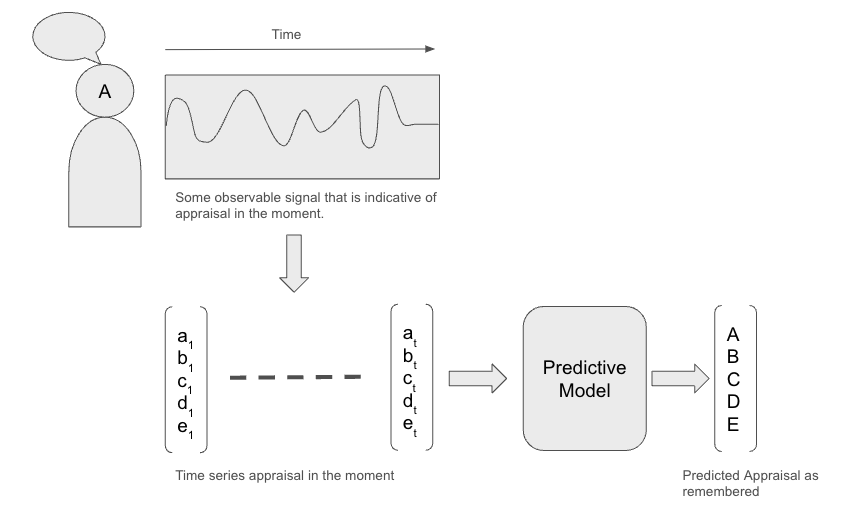
\includegraphics[width=\linewidth]{Images/schematic1.png}
    \caption{Schematic Representation of Situational Interdependence Prediction Model}
    \label{fig:model_diagram}
\end{figure}

\subsection{Dataset}
This research employs two distinct datasets: the PACO dataset \cite{matej2022designing} and the Negotiation dataset \cite{recorgnizing2021Dudzik}. Although they were collected for different purposes, both datasets provide comparable information relevant to our research aims. This includes audio-visual recordings of participants engaging in conversations from similar angles, along with post-conversation SIS measurements. In short, conversation records under the listed five contexts were present in the two datasets.

\begin{enumerate}
    \item Joint trust task setting (TRUST)
    \item Joint competence task setting (COMP)
    \item Feud Task setting (FEUD)
    \item Low conflict Negotiation setting (LConf)
    \item High conflict Negotiation setting (HConf)
\end{enumerate}

% explanation of paco
The PACO dataset \cite{matej2022designing} was initially developed to model partner selection and explore its relationship with human impressions during social interactions \cite{matej2022designing}. The dataset includes recordings of 3-minute online conversations between two individuals over three different contextual settings. The settings include performing 1) a joint trust task (TRUST), which is a cooperative decision-making task with mixed motives, 2) a joint competence task (COMP), where the outcome depends on the competence of two individuals, and 3) a Feud Task (FEUD), where facilitation of collaboration and active communication are important for the best outcome. Half of the participants were selected for performing the joint trust task and the other for the joint competence task. The feud tasks were performed by all participants. Each participant was asked to have one-on-one online video conversations for the two tasks with 3-5 other participants and to fill out a questionnaire including a 10-item version of questions from SIS after each conversation.

% Explanation of negotiation dataset
The other dataset is the Negotiation dataset \cite{recorgnizing2021Dudzik}. It contains recordings of negotiation conversations in face-to-face settings between two individuals. One of the participants was assigned to the "applicant" and the other to the "HR manager", where the latter has more power in the setting. The conversations are assigned to one of two conditions in terms of the intensity of conflict. The low conflict situation (LConf) has more options, five out of five options, which leads to a preferred outcome of both of them while the high conflict situation (HConf) has only one option and the rest leads to a consequence where one's best outcome is the other's worst outcome. Participants needed to carry out the 5-minute negotiation three times and fill out a survey that included a 10-item version of SIS, the same set of questions with the PACO, after each session. After the third session, they had to come up with an agreement and failure to do so had a consequence of either 60\%, 40\%, or 20\% of an even split.

\subsection{Modelling appraisal in the moment}
% % Valance, Arousal from non-textual verbal cue
% As mentioned in the section \ref{intro}, one of the overlapping dimensions of the appraisal process and situation perception is valance, which is the extent of how positively an individual perceives a situation. It can also be expected that the dominance, which is one of an outcome or indication of the appraisal process, could be reflective of the actual power that an individual has in a conversation, which is also one of the determinants of situational interdependence, which is found to be predictable from non-verbal cue \cite{recorgnizing2021Dudzik}. There is evidence that valance can be extracted from speech signals. In this research, a model for dimensional speech emotion recognition is going to be used \cite{wagner2023dawn} to exploit non-textual verbal cues. This model is based on pre-trained wav2vec 2.0 \cite{Baevski2020Advances}, which processes the input audio file into frozen CNN first and then the inner Transformer layer is fine-tuned to output a learned representation. It is then used to extract emotional dimensions of valance, arousal, and dominance by being trained on MSP-Podcast \cite{Lotfian2019building}. The implementation is available on Github \footnote{https://github.com/audeering/w2v2-how-to}. The limitation here is that the emotional expressions observed in the speech signal might not reflect the actual internal states or power distribution of an individual, thus here we assume that it is the case. 

% LLM are used to model appraisal in the moment in terms of SIS. 
As mentioned earlier in Section \ref{app_model}, the usage of LLM has been attempted previously in modelling emotional appraisal from textual content. This research is also going to follow this trend of using LLM to model the appraisal in the moment by looking at the textual conversation contents. Since the dimensions of the appraisal as remembered are in terms of the situational interdependence scale (SIS), the modelling of appraisal in the moment will also be in terms of the SIS. 

% The query has two types, 1) task definition 2) query
In formulating the prompt to model appraisal in the moment, we adopt a methodology similar to that of \citeauthor{feng2023affect}\cite{feng2023affect}. Their study is particularly relevant as it specifically addresses conversation settings. We incorporate two types of prompts: task definitions and queries. It's worth noting that \citeauthor{feng2023affect} also experimented with in-context learning; however, due to the absence of ground truth labels for appraisal dimensions in the moment in the datasets, we are unable to utilize this aspect in our setup. The task definition involves outlining each dimension of situational interdependence and describing the contextual setting. 

% The appraisal modelling takes place per utterance. Once it is evaluated, it is added to the conversation history for the next utterance query.
Meanwhile, the structure of the query prompt draws inspiration from \citeauthor{feng2023affect}\cite{feng2023affect}, with a focus on the process of appraisal estimation for each new utterance while maintaining the history of the conversation as context for future queries. The utterance of the conversation partner is also added to the conversation history. The example prompt is shown in Table \ref{tab:prompts}.

\begin{table}
    \centering
    \begin{tabular}{|p{3cm}|p{7cm}|} \hline
         Prompt type & Prompt template \\ \hhline{|==|}
         Task Definition & Consider the following list of concepts, called "Situational Interdependence" : [Mutual Dependence : (definition), Conflict of Interest : (definition), ...]\\ \hline
         Query & Given the dialogue history between PersonA and PersonB : [PersonA: ..., PersonB: ..., ...], what is the "Situational Interdependence" in the next utterance of PersonA "..."? \\ \hline
    \end{tabular}
    \caption{Templates of prompts for modelling appraisal in the moment. }
    \label{tab:prompts}
\end{table}

% The formulation of the prompt to model the appraisal dimensions using the Likert scale is inspired by several research \cite{feng2023affect, zhan-etal-2023-evaluating}. Out of the relevant papers which are found so far \cite{broekens2023fine, tak2023gpt, yongsatianchot2023investigating, zhan-etal-2023-evaluating}, \citeauthor{feng2023affect}'s experiment \cite{feng2023affect} seems to the closest settings to our experiment. They processed each utterance to identify emotions from a set of emotional labels within a conversational context, providing valuable inspiration for our study. 

\subsection{Predictive model}
The predictive model takes the time-variant appraisal in the moment in terms of situational interdependence as its input and the predicted values of appraisal as remembered in terms of situational interdependence as its output. To maintain the time-variant nature of appraisal for prediction, we utilize the Long Short-Term Memory network (LSTM). The LSTM's ability to capture long dependencies over time is well-suited for our task. To address RQ1, all instances of data are utilized, whereas for RQ2, a new network is trained for each contextual setting.

% Maybe Randomforest too but need to find papers
% Maybe Reinforcement learning too but need to find papers


% https://inria.github.io/scikit-learn-mooc/python_scripts/dev_features_importance.html

% Some ideas for the models
% Tim's paper
\section{Discussion}

\subsection{Limitations}
A combination of different modalities has more information regarding modelling appraisal in the moment \cite{hall2007sources}.

\bibliographystyle{ACM-Reference-Format}
\bibliography{ref}

\end{document}
